%\documentclass[letterpaper, paper,11pt]{AAS}
\documentclass[journal ]{new-aiaa}
\usepackage[utf8]{inputenc}
\usepackage{textcomp}
\usepackage{amsmath}
\usepackage{graphicx}
\usepackage[version=4]{mhchem}
\usepackage{siunitx}
\usepackage{longtable,tabularx}
\setlength\LTleft{0pt} 
%\newtheorem{theorem}{Theorem}
%\newcommand{\deg}{\ensuremath{^{\circ}}}
\newcommand{\state}{\ensuremath{\mathbf{x}}}
\newcommand{\control}{\ensuremath{\mathbf{u}}}
\newcommand{\ur}{\ensuremath{u_{\mathrm{ref}}}}
\newcommand{\State}{\ensuremath{\mathbf{X}}}
\newcommand{\Control}{\ensuremath{\mathbf{U}}}
%\newcommand{\costate}{\mathbf{p}}
%\newcommand{\multiplier}{\mathbf{\lambda}}
\newcommand{\param}{\ensuremath{\mathbf{p}}}
%\newcommand{\costate}{\mathbf{\lambda}}
%\newcommand{\multiplier}{\mathbf{\nu}}
\newcommand{\E}[1]{\mathbb{E}\left[#1\right]}
\newcommand{\V}[1]{\mathbb{V}[#1]}
\newcommand{\mean}{\mathbf{m}}
\newcommand{\cov}{C}
\newcommand{\std}{S}
\newcommand{\sample}{\ensuremath{\mathbf{z}}}
% Title Page
\title{Mars Entry Guidance for High Elevation Landing via Optimal Control Under Uncertainty}


\begin{document}
\author{Connor D. Noyes\thanks{Ph.D. Candidate, Department of Mechanical and Aerospace Engineering, University of California, Irvine, 92697} \ and Kenneth D. Mease\thanks{Professor Emeritus, Department of Mechanical and Aerospace Engineering, University of California, Irvine, 92697}}
\maketitle

% Refences with notes:
% AltitudeUnderUncertainty
% MarsEntryDesensitized % linearized but closed-loop with fixed gain. No consideration of saturation 
% EntryOUU % Does not use linearization, also doesnt solve in a conventional way, maybe remove?
% TrajectoryDesensitization % Desensitized like seywald and kumar, is it entry applied?
% EntryOUUThesis1 % Earth EDL, focuses on footprint computation, only considers open-loop in the reentry problem, and did not conduct monte carlo to confirm
% EntryOUUThesis2 % LQR, minimum control effort objective which stays away from the bounds, angle of attack as control variable. Does perform Monte Carlo(s) to validate improvement. 

%Rather than impose a chance constraint to reduce saturation, the control is freely allowed to saturate as long as the end result is good. 

% Ideas to discuss:
% Result of optimization is a reference trajectory and (linear) controller with desirable robustness 
% Demonstrate correlation between UT and MC results to validate use of the UT, but there are limits 
% Joint optimization (naturally) leads to superior results over fixed gains 
% Examine how solutions change with weights, and also initial state vs parametric uncertainty 
% Conclusions? New approach to combined reference + controller design 

% Mease notes to implement:
% discuss why velocity is the IV (removes constraint + better DDP convergence)
% Better discussion of how MSL/M2020 do their guidance design 

\section*{Abstract}
%The current generation of Mars entry vehicles employ a modified Apollo entry guidance that performs range control until a fixed velocity, and key trajectory metrics are the total range error and altitude at parachute deploy. We pose the entry guidance problem as an optimal control problem under uncertainty with closed-loop dynamics to determine a reference trajectory that is optimal with respect to an objective that weights mean altitude, altitude variance, and distance variance. The result is a reference trajectory with optimal margin for a given set of input dispersions. The robustness and optimality are validated in a Monte Carlo analysis. Novel aspects of the approach include use of the unscented transform to account for saturation in the closed-loop system, and the use of differential dynamic programming to solve the challenging nonlinear optimal control problem. 
\section*{Introduction}
%The first paragraph is about the future mission requirements driving entry guidance. 

%The second paragraph reviews the state-of-the-art and identifies potential limitations for meeting the new requirements. 

%Then the next paragraph will present the purpose of the paper, namely to present the proposed method, how it may lead to improvements, and how it will be tested. 
\lettrine{M}{aximizing} the altitude at the termination of the entry phase is of interest to both current and next generation Mars missions. The entry phase may be terminated at a fixed velocity \cite{MSL_EDL2}, at a fixed downrange distance \cite{TriggerComparison2020}, or by a more complex function of the vehicle state \cite{LuAdaptiveEDL}. Maximizing altitude at a terminal entry state allows the vehicle to target landing sites at higher elevations, which are motivated by reasons of scientific interest, by increasing the time available for subsequent descent and landing operations, which is particularly important in high ballistic coefficient vehicles. However, despite the importance of maximizing terminal altitude, missions must generally also consider additional objectives, such as reducing the size of the landing footprint. Often these multiple objectives are competing, as for example was the case on Mars Science Laboratory (MSL) mission, where the entry guidance designers noted that landing site elevations above -1 km (relative to the Mars aeroid surface) will induce a larger landing ellipse \cite{MSL_EDL2}. 
Future missions, including sample return \cite{MSR} and manned, will place even greater emphasis on robust performance than the current generation, such as pinpoint landing requirements \cite{EvolvableMars}. 
% TODO: Talk about altitude maximization references here 
The problem of maximizing the terminal altitude of Mars entry vehicles has been studied in a deterministic setting including indirect approaches based on Pontryagin's maximum principle
%\cite{AltitudeOptimization} % this one "proves" the switch numbers 
\cite{AltitudeOptimization,AltitudeOptimizationIndirect}, and an optimization-based onboard trajectory planning method based on a low-order parametrization designed to achieve high altitude at chute deploy
\cite{GuangfeiDissertation}. 
%Typically these papers consider predictive guidance and use parametrizations of the bank angle designed to yield high altitudes. 
Altitude maximization has also been studied in an uncertain setting in \cite{AltitudeUnderUncertainty}, where the objective was to maximize a function of the mean and standard deviation of altitude, and in \cite{MarsEntryDesensitized}, where the objective was to maximizing the terminal altitude while penalizing sensitivity terms related to variations in the initial state.

The state-of-the-practice for Mars entry vehicles is represented by Mars 2020, which inherited its entry guidance architecture from Mars Science Laboratory (MSL) \cite{M2020_EDL}. One change from MSL is that Mars 2020 will trigger parachute deployment based on a range trigger instead of a velocity trigger \cite{TriggerComparison2020}.
The guidance design method used on these latest Mars entry vehicles \cite{MSL_EDL2,M2020_EDL} can be divided into two steps. The first step is to design a reference bank profile and compute the corresponding reference trajectory via open-loop simulation. In the second step, a feedback control law is chosen, and closed-loop performance using the reference trajectory is evaluated under off-nominal conditions. The free parameters (if any) of the guidance algorithm are then tuned until the performance is satisfactory. If the necessary performance cannot be achieved through tuning, the reference trajectory is changed and the process is repeated. 
%This design cycle may be viewed as an inner loop, in which Monte Carlo simulation is used to quantify off-nominal performance, and the outer loop in which the entry guidance designer adjusts the reference trajectory based on the results. 
MSL and Mars 2020 both chose the entry terminal point controller \cite{MSL_EDL, M2020_EDL}, a modified version of the Apollo second phase guidance \cite{MSL_EDL2}. Because the guidance gains are determined by the reference trajectory in this guidance algorithm, proper design of the reference is the most important part of the guidance design. The reference bank angle profile is parametrized using an early bank angle, a late bank angle, and the velocities at which the linear (in velocity)) ramp from early to late bank angle begin and end. This variable bank angle profile was a modification from the original Apollo algorithm, which assumed a constant bank angle reference profile. This change allows for more flexibility in trajectory design including enabling higher parachute deploy altitudes \cite{MSL_EDL2}.
%The free parameter affecting range performance is the range overcontrol gain, a multiplier on the predicted range error. 

As with MSL, we consider the guidance approach as bank angle modulation using reference trajectory-based feedback control. In this work we present an alternative method for reference trajectory design. It is produced by trajectory optimization accounting for both the feedback control law and the uncertainties affecting the problem. This approach blends optimal control with uncertainty quantification to incorporate statistical uncertainty in the vehicle initial state and model parameters, such as ballistic coefficient or atmospheric density. As a result, the terminal entry state is given by a joint distribution rather than a single nominal point, and statistics of the distribution may be used in the optimization objective. While MSL did not optimize an objective function, the goal of the reference trajectory design was to balance the lift of the vehicle to reduce range error while achieving a safe parachute deploy altitude \cite{MSL_EDL2}. In order to achieve these goals, the objective function in this work includes mean altitude and a weighted combination of altitude standard deviation, and downrange standard deviation. For any choice of weights on these standard deviations, we minimize the objective over piece-wise constant bank profiles with many segments to allow for more general profiles. In the same way that MSL expanded the bank angle profiles under consideration to meet mission requirements, this is a natural extension to meet the stringent requirements of future missions. This means that our design parameters are the weights associated with altitude standard deviation and range standard deviation rather than the parameters of the reference bank profile. 
%The effect of these weights on the terminal altitude and range distributions is more intuitive than the effect of adjusting components of the reference bank angle profile. 
%Use of optimal control to determine the bank profile removes the designer from the loop.  
% TODO: Talk about optimization under uncertainty here?

% TODO:
% Notes from phone call:
 %DDP and UT make it feasible to optimize all at once 
% The objectives aren't new; but we're tackling them in a new, precise, efficient way
In the MSL design method, a number of stress trajectories are simulated in closed-loop using the reference trajectory and entry terminal point controller gains to estimate off-nominal performance prior to Monte Carlo simulation \cite{MSL_EDL2}. This provides the designer some information at a reduced computational cost. In this work, we use the unscented transform (UT) \cite{UT1997} instead of stress cases to estimate performance prior to Monte Carlo simulation. The unscented transform is a deterministic sampling-based method that propagates a set of sigma points through the nonlinear dynamics and reconstructs the mean and covariance from the transformed samples. In order to validate the performance of the reference trajectories designed using the UT-estimated statistics, closed-loop Monte Carlo simulations are conducted.

Optimal control approaches that weight a nominal optimization objective with covariance terms have been studied in the context of entry guidance, including \cite{AltitudeUnderUncertainty, MarsEntryDesensitized, EntryOUUThesis1, EntryOUUThesis2, EntryOUU}.
Reference \cite{AltitudeUnderUncertainty} is perhaps the most closely related method to our work. The first important distinction is the multi-objective formulation in this work additionally considers the downrange standard deviation, rather than strictly focus on altitude. Additional differences of our approach include the use of the unscented transform in place of linear covariance propagation, and the inclusion of the feedback control law to optimize closed-loop performance rather than open-loop performance. Reference \cite{AltitudeUnderUncertainty} also considered constraints on heat flux and dynamic pressure which are not considered in this work. 
%Accounting for the feedback controller and uncertainties during the reference trajectory design eliminates the iterative two-step process. By considering more general reference controls generated via optimal control, improved performance is expected relative to the low-order parametrization used by MSL.

Optimal control under uncertainty adds an additional layer of computational complexity. Using the UT results in a challenging optimal control problem in many state variables. In this work, the large-scale problem is solved using differential dynamic programming (DDP) \cite{DDP}. DDP is a shooting method originally devised to solve unconstrained nonlinear optimal control problems that has since seen numerous extensions, including to constrained problems \cite{DDP_ControlLimited,HDDP1,HDDP2,DDP_NonlinearConstraints,DDP_InteriorPoint}, and stochastic problems \cite{iLQG, DDP_Stochastic, ozaki_UT,ozaki2020tube}. 
%A common theme among all of these references is their application to robotics \cite{iLQG, DDP_Stochastic} or low thrust trajectory optimization \cite{HDDP1,HDDP2,ozaki_UT,ozaki2020tube}. Despite the apparent success in these fields, 
Despite its apparent success in robotics and low-thrust trajectory optimization, DDP has not yet garnered much attention in the entry guidance community. 
%Simultaneous transcription methods, especially collocation methods, are popular for their ability to readily handle nonlinear constraints on states and controls, and indeed for deterministic problems with low state dimension, their applicability and effectiveness is undeniable. In a stochastic setting, however, the most common methods of converting the problem to a deterministic one involve an increase in the dimensionality of the state vector that render the problem difficult to solve this way. Meanwhile, DDP is an effective method for solving large-scale optimal control problems. 


% Use of samples, in particular the unscented transform, addresses the issue of uncertainty quantification in the presence of control saturation, a key issue in Mars entry guidance that has not been discussed in the context of variance reduction.

%A unifying theme of the previous literature on mean-variance control is the use of linear propagation to estimate the mean state and state covariance, which we argue are insufficient for the problem at hand. 

 
% and superior performance can be achieved relative to design methods currently in practice.



%\subsection*{Related Work}
%\subsubsection*{Altitude Maximization}
%The motivation behind altitude maximization in Mars entry is to provide sufficient timeline for subsequent descent and landing operations. The problem of maximizing the terminal altitude of Mars entry vehicles has been studied in a deterministic setting
%\cite{AltitudeOptimization} % this one "proves" the switch numbers 
%\cite{AltitudeOptimizationIndirect}
%\cite{GuangfeiDissertation}
%and also in a stochastic setting \cite{AltitudeUnderUncertainty} where linear covariance techniques were used to reduce open-loop covariance, and in \cite{MarsEntryDesensitized} sensitivity terms related to variations in the initial state are considered.

%\subsubsection*{Optimal Control with Sensitivity/Covariance Reduction}
%The literature on optimal control problems that weight a nominal optimization objective with covariance or sensitivity terms is vast, and the idea has seen a large amount of attention within the entry guidance community including \cite{AltitudeUnderUncertainty, MarsEntryDesensitized, EntryOUUThesis1, EntryOUUThesis2, EntryOUU}.
%The focus has been on making open-loop trajectories more robust, regardless of whether the loop will be closed for the real system. This focus on open-loop strategies is one reason why the issue of control saturation has not been adequately addressed. An additional reason is the (nominal) optimization objective under consideration: altitude optimal trajectories are known to be bang-bang \cite{AltitudeOptimization} while other objectives such as maximum crossrange trajectories, studied in \cite{EntryOUUThesis2}, are not.  

%One common feature of these studies is the use linear propagation techniques to compute sensitivity matrices or covariance matrices, which we will demonstrate is insufficient for closed-loop optimization in the presence of control saturation. Our use of the unscented transform allows us to accurately capture the effects of saturation on performance. Although the unscented transform has been used in the context of optimal control under uncertainty \cite{UnscentedOptimalControl}, the focus remained on open-loop strategies. 

%While a number of these reports note the possibility of closed-loop covariance reduction, only \cite{MarsEntryDesensitized}, where the linear approach to uncertainty quantification is used with a fixed gain matrix, and \cite{EntryOUUThesis2}, where the Linear Quadratic Regulator (LQR) approach is used, actually examine this scenario, and both apply the linear approach to uncertainty quantification.

%\subsection*{Contributions}


%As a second contribution, we demonstrate that differential dynamic programming is a natural choice for solving the nonlinear optimal control problem because the method scales favorably in state dimension compared to the collocation methods utilized in other covariance reduction methods. Despite its popularity in robotics and low thrust trajectory applications, DDP has seen virtually no application in entry trajectory optimization. 

%More concretely, consider an optimal control problem in which the system is described by $n$ states, $m$ controls, and discretization of the independent variable into $N$ stages. In an uncertain setting, the most common ways to incorporate distribution information involve including $n\times n$ sensitivity terms, or $\frac{n(n+1)}{2}$ covariance terms, or use sample-based approximations in which the state dimension with $S$ samples yields state dimension $Sn$. This increased state dimension poses fewer problems in DDP, which iteratively solves $N$ optimization problems in $m$ variables, compared to direct methods, which solve a single large-scale problem in $N(n+m)$ variables.

%In entry guidance problems, performance is characterized by extrema of one or more quantities of interest, e.g. trajectories with low altitude or high Mach number at parachute deployment. Altitude optimal trajectories are bang-bang in nature, and leave no margin for feedback control. The amount of margin that ought to be left is a function of the system uncertainty and the guidance algorithm chosen to correct off nominal performance. Clearly, then, for a fixed uncertainty set and guidance algorithm, there exists an optimal tradeoff between mean performance, and tail performance of closed-loop cases. Our goal is to compute such an optimal reference trajectory and margin. 

%One way to characterize the distribution of a quantity is with its mean and variance, which motivates propagation of these moments as an efficient alternative to propagating the entire distribution. The most efficient method is linear propagation; for linear systems with Gaussian distributed uncertainty the result is exact, but for nonlinear systems the method can be inaccurate. The unscented transform is a deterministic sampling-based method that propagates a set of sigma points through the nonlinear dynamics and reconstructs the mean and covariance from the transformed samples.

%Typical trajectory optimization designs a reference trajectory that can be utilized in different ways to achieve the guidance objective. However, the optimality of this reference trajectory is directly at odds with robust closed-loop performance for several problems of interest in entry guidance: altitude maximization and propellant minimization.  

%\section{Terminology: Uncertain vs Stochastic}
% Stochastic optimal control is concerned with systems governed by stochastic differential equations
% \begin{align*}
% \mathrm{d}\state = f(t,\state)\mathrm{d}t + g(t,\state)\mathrm{d}w
% \end{align*}
% where $w$ is a Standard Brownian motion and the initial state may be given by a distribution or a single state. The problem is subject to the rules of stochastic calculus and the partial differential equation (PDE) governing the evolution of the probability density of the state vector is the Fokker-Planck equation. 
% 
% In contrast, uncertain optimal control concerns systems governed by ordinary differential equations with initial conditions governed by a distribution, and the PDE that governs the probability density evolution is the Liouville equation.

%In both types of problems, the objective function is expressed probabilistically, often via expectations and variances, and constraints are incorporated as chance constraints. 

%The distinction has the following impact on SDDP algorithm: all terms related to diffusion term vanish, and the forward/backward simulations are conducted without noise. In Ozaki's approach, the backward pass computes expectations of the derivative terms. In constrast, we compute deterministic derivatives with respect to the extended state vector, and only compute the expectations in the cost function. 

%In our approach, samples are propagated through the full nonlinear dynamics, and the moments are computed from a finite set of samples $\sample_i,\,i=1,...,N$:
%\begin{align}
%\mean &\approx N^{-1}\sum_{i=1}^{N} \sample_i \\
%\cov &\approx N^{-1}\sum_{i=1}^{N} (\sample_i-\mean)(\sample_i-\mean)^T
%\end{align}

\section*{Entry Trajectory Design Problem}
The problem of designing a reference entry trajectory is posed as an optimal control problem under uncertainty. Following the approach taken by MSL and M2020, only the longitudinal motion is accounted for in the reference trajectory design. To complete the entry guidance design, separate lateral guidance logic determines when bank reversals should be commanded to prevent large crossrange distances to the target. The lateral guidance problem is not considered here.
%TODO: Say that lateral guidance is not considered in the intro as well per Mease's suggestion 

The longitudinal equations of motion of a point-mass model of a Mars entry vehicle are written with respect to the planet-relative vehicle velocity magnitude, and the state vector $\state=[h,\,\gamma,\, s]^T$ consists of the vehicle altitude about the planet surface, the flight path angle, and the downrange distance flown. The entry trajectory terminates at a fixed velocity $v_f$. Using velocity as the independent variable removes the need to enforce a constraint on the terminal velocity. The scalar control variable $u=\cos\sigma$ where $\sigma$ is the bank angle, and thus the dynamics may be written
\begin{align}
h' &= \frac{v\sin\gamma}{-D - g\sin\gamma} \label{eq_dynamics_altitude}\\
s' &= \frac{v\cos\gamma}{-D - g\sin\gamma} \\
\gamma' &= \frac{\frac{L}{V}u + \left(\frac{v}{h+r_p}-\frac{g}{v}\right)\cos\gamma}{-D - g\sin\gamma} \label{eq_dynamics_fpa}
\end{align}
where $(\cdot)' = \frac{d\cdot}{dv}$, $r_p$ is the planet radius, $g=\mu/(h+r_p)^2$ is the magnitude of the gravitational acceleration, and the lift and drag accelerations are
\begin{align}
D = \frac{1}{2}\frac{\rho}{\beta} v^2 \\
L = D(\frac{L}{D})
\end{align}
where $\rho=\rho_0\exp\left(-\frac{h}{h_s}\right)$ is an exponential model of the atmospheric density, $\beta=\frac{m}{C_DS}$ is the ballistic coefficient, $m$ is the vehicle mass, and $L/D$ is the lift-to-drag ratio.
The initial state vector is assumed to be governed by a distribution with known first two moments
 \begin{align}
 \E{\state(v_0)} = \state_0 \label{eq_ic_mean}\\ 
 \V{\state(v_0)} = \cov_0 \label{eq_ic_cov}
 \end{align}
In this work, we assume the initial state is distributed according to $\state(v_0)\sim N(\state_0,\,\cov_0)$, but the assumption of normality is not required.

To account for the effects of the control law, the control $u$ consists of both a reference control $\ur$, and a feedback term $\delta u$, in contrast to open-loop design methods where $u=\ur$. 
The control law is assumed to be to a saturated linear state feedback 
\begin{align}
u(v,\state) &= \mathrm{sat}_{[0,1]}\left(\ur(v) + \delta u(v,\state)\right)\\
\delta u &= k_D\delta D + k_{\gamma}\delta\gamma + k_s\delta s \label{eq_feedback}
\end{align}
where we note that, consistent with state-of-the-art EDL operations on Mars, drag acceleration has been used as a feedback term in place of altitude. The gains $k_i$ may be functions of velocity, and the saturation function is defined
\begin{align*}
\mathrm{sat}_{[a,b]}(x) = \left\{\begin{array}{lc}
        a, &  x < a\\
        x, &  a\le x \le b\\
        b, &  b < x
        \end{array} \right. % The period stops a warning about not closing the left 
\end{align*}
The saturation function is required to ensure that, regardless of the value of the reference control \ur, the closed-loop control $u(v,\state)$ always satisfies the control limits. Because the control variable is the cosine of an angle, its magnitude must be bounded by one. Due to the low lift capability of current generation Mars entry capsules, it may be prudent to further restrict the vehicle from bank angles that orient the lift vector downward, so in our application we apply
\begin{align}
	0 \le \ur(v) \le 1 \label{eq_control_bounds}
\end{align}
which disallows bank angle magnitudes greater than $90^\circ$.
The state deviations in Eq.~(\ref{eq_feedback}) are computed with respect to the mean state at the current velocity, e.g., $\delta D(v) = D(v) - \E{D(v)}$.
%Two scenarios will be considered. In the first, only the open-loop control $u_0$ is determined by the optimal control solution; the feedback gains are not included as optimization variables, but may still be functions of the planned trajectory, as in e.g. Apollo guidance, which computes influence coefficients around a nominal trajectory. In this setting, DDP searches for the most robust path subject to a given guidance approach. In the second scenario, the gains are included as controls to be determined via DDP. 

The optimal control problem is to determine the piece-wise constant reference control $\ur\left[v_0,v_f\right]$ that minimizes the objective functional
\begin{align}
%J &= -\E{h(v_f)} + w_h\V{h(v_f)}^{\frac{1}{2}} + w_s\V{s(v_f)}^{\frac{1}{2}}.
%J(\ur\left[v_0,v_f\right]) &= -\E{h(v_f)} + w_h\sigma_h(v_f) + w_s\sigma_s(v_f) \label{eq_objective}
J &= -\E{h(v_f)} + w_h\sigma_h(v_f) + w_s\sigma_s(v_f) \label{eq_objective}
\end{align}
subject to the equations of motion $(\ref{eq_dynamics_altitude})-(\ref{eq_dynamics_fpa})$, the initial conditions~(\ref{eq_ic_mean})-(\ref{eq_ic_cov}), and the bounded control (\ref{eq_control_bounds}). 
In addition to the mean altitude component, a weight $w_h\ge0$ multiplies the altitude deviation and thus allows for additional emphasis on maximizing a measure of the low end of the distribution. Additionally, while the mean downrange distance is unconstrained, there is a penalty $w_s\ge0$ on standard deviation of the downrange distance. For small $w_s$, this term is used to discourage solutions from sacrificing downrange accuracy for small altitude improvements. Larger weights encourage greater reduction in downrange errors at the expense of altitude performance. The solution consists of the reference controls and the reference trajectory.
%There are no terminal constraints.

\subsubsection*{Remark} Either variances or standard deviations may be used in Eq.~(\ref{eq_objective}). In practice, appropriate choices of the weights can produce equivalent results, but standard deviations are preferred because they are in the same units as the state variables, and allow for more natural interpretations of the weights. An additional consideration is that the square root is not differentiable at zero, but both in theory and in practice, the terminal standard deviations are never exactly zero since the covariance matrix is positive definite.
\subsubsection*{Remark} Uncertainty in the parameters in governing differential equations can be included by appending the parameters $\param$ to the state vector with trivial dynamics, $\param'=\bf0$.
%In summary, the optimal control problem under consideration is 
%	\begin{align}
%	\min_{\ur\left[v_0,v_f\right]}\ J\\  % 
%	\mathrm{subject\,to\,} \nonumber\\ 
%	&\mathbf{\state'} = f(v,\state,\ur) \\
%	&\E{\state(v_0)} = \state_0 \\
%	&\V{\state(v_0)} = \cov_0 \\
%	&0 \le \ur(v) \le 1 
%	\end{align}

\section*{Optimal Control Solution via Unscented Transform and DDP}
A key issue in solving the optimal control problem is computing the expected values and standard deviations in the objective functional and feedback terms. Broadly, uncertainty quantification (UQ) methods trade between accuracy and the amount of computation required. For example, linear covariance propagation is one of the most efficient UQ methods for computing the first two probability moments, but its accuracy depends on the nonlinearity of the system dynamics. At the other extreme, Monte Carlo simulation can estimate higher order moments to arbitrary accuracy, but may require a huge number of samples in order to do so. Since UQ will be performed at each optimal control solver iteration, the method chosen must strike a careful balance these two aspects. For very fast but inaccurate methods, the solution may not perform as expected in a higher fidelity UQ, such as Monte Carlo simulation, and the benefit of the approach may be diminished or lost entirely. On the other hand, slow but accurate methods will result in very long solution times. In this work, the unscented transform (UT) \cite{UT1997} is chosen to compute the required statistics. The UT is preferable to linear covariance techniques because the sigma points are propagated through the full nonlinear, saturated dynamics, and are thus able to capture their effects on the distribution more accurately than linearization. 
%While random sampling can produce more accurate estimates than either linear propagation or the unscented transform,
It is also preferable to random sampling because the number of sigma points is generally lower than the number of samples required for equivalent precision, and the sigma points are given deterministically by the UT algorithm. %TODO: citation?

Next, because control saturation is a key issue in the closed-loop dynamics, the control-limited box-DDP algorithm \cite{DDP_ControlLimited} is employed to solve for the control updates during the backward pass. While this approach results in reference controls that satisfy the control limits, the saturation function is required in the forward integration to ensure the closed-loop sigma point trajectories also respect the control limits.

\subsection*{Unscented Transform}
The unscented transform is a method to approximate the first two moments of a nonlinear transformation of a probability distribution. Consider a scalar quantity $q\in\mathbb{R}$ given by a nonlinear transformation $q = F(\param)$ of a vector $\param\in\mathbb{R}^n$ with known mean and covariance
\begin{align*}
\E{\param} &= \bar{\param}\\
\V{\param} &= \cov_{\param}
\end{align*}
A set of $2n+1$ sigma points and associated weights are computed 
\begin{align*}
\param_0 &= \bar{\param} \\
\param_i &=  \bar{\param} + \left(\sqrt{\alpha \cov_{\param}}\right)_i \\
\param_{i+n} &=  \bar{\param} - \left(\sqrt{\alpha\cov_{\param}}\right)_i \\
w_0 &= \frac{\beta - n}{\alpha} \\
w_i &= w_{i+n} = \frac{1}{2\alpha}
\end{align*}
where $\alpha$ is a scaling parameter, and $\left(\sqrt{\alpha \cov_{\param}}\right)_i$ is the $i^{\mathrm{th}}$ column of the matrix square root of $\beta \cov_{\param}$. The sigma points are then mapped through the transformation
\begin{align}
q_i = F(\param_i),\;\;i=0,...,2n
\end{align}
and finally, the mean and variance are approximated using the weights and transformed sigma points
\begin{align*}
\E{q} &\approx \sum_{i=0}^{2n}w_iq_i  \triangleq \bar{q}\\
\V{q} &\approx \sum_{i=0}^{2n}w_i\left(q_i - \bar{q}\right)^2
\end{align*}

\subsection*{Control-Limited Differential Dynamic Programming}
In this section we review the differential dynamic programming method that will be used to solve the optimal control problem. 
The algorithm is formulated in discrete time, so the continuous time dynamics must be discretized, e.g., using Euler integration:
\begin{align}
\state_{i+1} = \mathbf{f}(v, \state_i,\control_i) = \state_i + \state_i'\Delta v \label{eq_discrete_dynamics}
\end{align}
A trajectory $\{\State,\Control\}$ is a sequence of controls $ \Control=\{\control_0,\control_1,...,\control_{N-1}\} $ and corresponding states $\State=\{\state_0,\state_1,...,\state_N\}$ determined by integrating (\ref{eq_discrete_dynamics}) from $\state_0$.
Although the optimal control objective as posed considers only a terminal cost, in this section we consider a generic cost function $J$ consisting of a sum of running costs $l$ and a terminal cost $l_N$:
\begin{align}
J(\state_0,\Control) = \sum_{i=0}^{N-1}l(\state_i,\control_i) + l_N(\state_N)
\end{align}
Let $\Control_i$ be the tail of the control sequence, $\{\control_i,\control_{i+1},...,\control_{N-1}\}$, and the cost-to-go $J_i$, defined as the partial sum of costs from $i$ to $N$ is
\begin{align}
J_i(\state,\Control_i) = \sum_{j=i}^{N-1}l(\state_j,\control_j) + l_N(\state_N)
\end{align}
The Value function at timestep $i$ is the optimal cost-to-go at \state
\begin{align}
V_i(\state) = \min_{\Control_i} J(\state, \Control_i)
\end{align}
and at the final timestep the Value function is equal to the terminal objective. The Dynamic Programming principle reduces the problem of minimization over $\Control_i$ to a sequence of minimization problems over $u$ at each timestep 
\begin{align}
V(\state) = \min_{\control}\left[l(\state,\control) + V^+(\mathbf{f}(\state,\control))\right] \label{eq_dynamic_programming}
\end{align}
where $V^+$ is the Value at the next time step.
Let the pseudo-Hamiltonian $Q(\delta\state,\delta\control)$ be the change in Value function as a function of perturbations to the pair $(\state,\control)$:
\begin{align}
Q(\delta\state,\delta\control) = l(\state+\delta\state,\control+\delta\control) + V^+(\mathbf{f}(\state+\delta\state,\control+\delta\control))
\end{align}
The second-order expansion of $ Q $ is given by
\begin{align}
Q_\state &= l_\state + \mathbf{f}_\state^T V^+_\state \\
Q_\control &= l_\control + \mathbf{f}_\control^T V^+_\state \\
Q_{\state\state} &= l_{\state\state} + \mathbf{f}_\state^T V^+_{\state\state}\mathbf{f}_\state + V^+_\state \mathbf{f}_{\state\state} \label{eq_hessian1}\\
Q_{\control\state} &= l_{\control\state} + \mathbf{f}_\control^T V^+_{\state\state}\mathbf{f}_\state + V^+_\state \mathbf{f}_{\control\state} \label{eq_hessian2}\\
Q_{\control\control} &= l_{\control\control} + \mathbf{f}_\control^T V^+_{\state\state}\mathbf{f}_\control + V^+_\state \mathbf{f}_{\control\control} \label{eq_hessian3}
\end{align}
where the subscripts denote partial derivatives with respect to that quantity, and the final term in each of the Hessian equations (\ref{eq_hessian1})-(\ref{eq_hessian3}) are tensor-vector contractions. %TODO: rewrite them as sums over the 'pages' of the hessian

\subsubsection*{Remark} The second derivatives $\mathbf{f}_{\state\state},\, \mathbf{f}_{\control\state}$ in Eq.~(\ref{eq_hessian1}),(\ref{eq_hessian2}) are $n\times n\times n$ and $m\times n\times n$ tensors, respectively, that must either be stored at $N$ timesteps, or else recomputed in the event the backward pass must be repeated with increased regularization. For large $n$, both computing and storing these quantities is problematic. Unfortunately, removing these terms entirely, as is done in the iterative Linear Quadratic Gaussian method \cite{iLQG}, leads to poor performance for the problem under consideration. In particular, the first-order algorithm has a noticeably smaller radius of convergence, and different guesses at the initial control sequence often lead to different local minima. In contrast, the full second-order DDP algorithm consistently converges to a single minimum from most guesses. Thus, we propose a compromise in which only the $n\times m \times m$ tensor $f_{\control\control}$ is retained in the above equations. Numerical experiments suggest this is sufficient to avoid poor solutions, at the expense of a slower convergence rate than the full algorithm with all second-order terms included. However, in the situation at hand, in which the number of controls $m$ is fixed and small ($ \le4 $), and the state dimension, which depends on the number of uncertainties under consideration, is large ($20 < n <60$), this modification proves to be enabling for $n\ge 30$ with $N=1000$. A limited-memory version of the Quasi-Newton approximations to these terms proposed in \cite{QNDDP} may also be a good choice to obtain superlinear convergence properties of the approximated second order algorithm while reducing the memory required. 
%(This reduces complexity from cubic in $n$ to linear)

The optimal control modification $\delta\control^*$ for some perturbation $\delta\state$ is a locally-linear feedback control $\delta\control^* = \mathbf{k} + K\delta\state$ obtained by minimizing the quadratic model subject to linear bounds on the controls
\begin{align}
\mathbf{k} = &\arg\min_{\delta\control} Q(\delta\state,\delta\control) \\
&\mathrm{subject\,to\,\;} \nonumber\\
\control_{\min}\le &\control+\delta\control \le\control_{\max}
\end{align}
and $K = -Q_{\control\control}^{-1}Q_{\control\state}$. Substituting the optimal control into the expansion of $Q$, a quadratic model of $V$ is obtained with derivatives
\begin{align}
\begin{split}
\label{eq_value_recurse}
V_\state &= Q_{\state}- K^TQ_{\control\control}\mathbf{k}\\
V_{\state\state} &= Q_{\state\state} - K^TQ_{\control\control}K.
\end{split}
\end{align}
The backward pass is performed by initializing $V$ and its derivatives with the value and derivatives of the terminal objective, then recursively computing the optimal control policy and (\ref{eq_value_recurse}).

The forward pass uses the newly computed control policy to integrate the new trajectory, subject to a backtracking line search
\begin{align}
\hat{\state}_0 &= \state_0 \\
\hat{\control}_{i} &= \control_i + \epsilon \mathbf{k}_i + K_i(\hat{\state}_i - \state_i)\\
\hat{\state}_0 &= f(\hat{\state}_i,\hat{\control}_i)
\end{align}
where $\epsilon$ is a search parameter initialized to 1 and reduced until the Value function shows improvement. The backward-forward iterations are repeated until convergence to a locally optimal trajectory. In the event 
%TODO: talk about regularization of the solution and failed backward passes.
\subsection*{Objective Reformulation}
In order for DDP to be applied to this problem for arbitrary $w_h,w_s\ge 0$, it is essential to reformulate some or all of the objective terms as running costs rather than terminal costs. This is because the terminal formulation results in singularity of the Hessian of the pseudo-Hamiltonian with respect to the control, and this quantity must be invertible for the algorithm to proceed. In practice, one could also add a small control regularization term to the objective, but experience has shown that reformulating the mean altitude objective is sufficient. Due to linearity of the expectation operator, we have the following relationships for the time rate of change of the first two moments
\begin{align}
\frac{d }{d t}\E{x} &= \E{\dot{x}} \\
\frac{d }{d t}\V{x} &= \E{2x\dot{x}} - 2\E{x}\E{\dot{x}} \\
\sigma_x &= \V{x}^{\frac{1}{2}} \\
\frac{d }{d t}\sigma_x &= \frac{1}{2\sigma_x}\frac{d }{d t}\V{x}
%\frac{d }{d t}\V{x}^{\frac{1}{2}} &= \frac{1}{2\V{x}^{\frac{1}{2}}}\frac{d }{d t}\V{x}
\end{align}
and thus running cost used in the reformulated objective function is 
\begin{align}
%J = \int_{v_0}^{v_f}-\E{h'} +  2w_h(\E{hh'}-\E{h}\E{h'}) + 2w_s(\E{ss'}-\E{s}\E{s'})\mathrm{d}v \\
%J = \sum_{i=0}^{N-1} \left[-\E{h'} +  2w_h(\E{hh'}-\E{h}\E{h'}) + 2w_s(\E{ss'}-\E{s}\E{s'})\right]\delta v 
l(\state,\control) = -\E{h'} +  2w_h(\E{hh'}-\E{h}\E{h'}) + 2w_s(\E{ss'}-\E{s}\E{s'})
\end{align}

\subsubsection*{Remark} While reformulating the mean altitude objective is essential to solving the problem, especially when $w_s=w_h=0$, reformulating the standard deviation terms is not. However, in numerical experiments we found that while both formulations result in the same solution, using running costs for the standard deviations allows DDP to converge in noticeably fewer iterations.

\subsubsection*{Remark} The non-differentiability of the saturation function in the controller also produces difficulties for the DDP algorithm, and thus we substitute the following smooth approximation when solving the optimal control problem
\begin{align*}
\mathrm{sat}_{[0,1]}(x) \approx \frac{1}{2} + \frac{1}{4K}\log\left(\frac{\cosh (2Kx)}{\cosh (2K(x-1))}\right) 
\end{align*}
where $K$ is a tuning parameter. $K=20$ in our implementation.
\subsubsection*{Remark}
Prior to solving the challenging optimal control problem under uncertainty, we applied DDP to altitude-optimal control without considering uncertainty. This was done so that we could verify it recovers the optimal bang-bang solutions, which could also be computed using a different method such as GPOPS-II\cite{GPOPS2}.

In addition to eliminating a terminal constraint, using velocity as the independent variable was also advantageous in solving the optimal control problem via DDP. Although we have not done a full analysis, one possibility is that, because DDP respects the temporal structure of the optimal control solution, this removes derivatives with respect to velocity. Because the aerodynamic accelerations are quadratic in velocity, this may have a large impact on the problem sensitivity. We also examined downrange distance as the independent variable, and found that convergence was poor unless a very close guess at the optimal control was used. In contrast to velocity, downrange distance does not appear in the equations of motion. 
%\section*{Uncertainty Quantification}
%Show that in the presence of saturation and with a closed-loop, linearization isn't appropriate. 
%
%\begin{table}[h]
%%\caption{Comparison between uncertainty quantification methods for open-loop simulations. Both the linear propagation and the unscented transform are quite close the Monte Carlo values.
%\begin{table}[h]
%    \begin{tabular} {|c|c||>{\centering}p{.9cm}|>{\centering}p{.9cm}|>{\centering}p{.9cm}|c|}
%        \hline
%        $Truth$ & $Predicted$ & ADA & SVM & GLM & Blended \\ \hline
%        T & T & 512 & 463 & 423 & 472 \\ 
%        T & F & 19  & 68  & 108 & 0   \\ 
%        F & T & 5   & 85  & 67  & 22  \\ 
%        F & F & 580 & 500 & 518 & 98  \\ \hline
%    \end{tabular} \\ \vskip .5cm
%
%    \begin{tabular} {|>{\centering}p{2.9cm}||c|c|c|c|c|}
%        \hline
%        $Accuracy Metric$ & ADA & SVM & GLM & Blended \\ \hline
%        Precision & 99.0\% & 84.5\% & 86.3\% & 95.5\% \\ 
%        Recall    & 96.4\% & 87.2\% & 79.7\% & 100\%  \\
%        Accuracy  & 97.8\% & 86.3\% & 84.3\% & 96.3\% \\ \hline
%    \end{tabular} 
%
%    \caption{Truth Tables and Accuracy Measures for each modeling library.}
%    \label{tab:truthTables}   
%\end{table}

\section*{Numerical Results}
A series of numerical experiments are conducted to illustrate the approach. The first section compares the presented approach to conventional reference trajectories designed by nominal optimal control and fixed bank angle margins. The second section investigates how the optimal trajectories change with the weights $w_h,\,w_s$, incorporating both initial state uncertainty and parametric uncertainty.
%The final set of numerical experiments compares the use of two different methods of generating time-varying gains tailored to the entry problem: linear quadratic regulator and modified Apollo guidance gains flown on MSL and Mars2020. Additionally, we validate our use of the unscented transform by comparison with Monte Carlo simulations.

All simulations are conducted on a five metric ton entry vehicle with a nominal $L/D=0.28$, i.e., in the same class as the Sample Retrieval Lander considered for the Mars Sample Return campaign \cite{MSR}. In order to contend with the issue that the entry velocity is not generally monotonically decreasing from the entry interface, we propagate the initial state and covariance matrix using time as the independent variable to the point where it does become monotonic and compute the mean and covariance at that point. The resulting nominal (or mean) entry state at $v_0 = 5525$ m/s is $x_0 = [54.5\,\mathrm{km},\,-11.5^{\circ}, 0\,\mathrm{km}]^T$. The initial state uncertainty around the mean is $\sigma_h = 2.5$ km, $\sigma_{\gamma} = 0.25^{\circ}$, $\sigma_s = 10$ km. Uncertainty is also modeled in the vehicle $L/D$ ratio, ballistic coefficient, and atmospheric density with $\sigma_{L/D} = 5\%$ km, $\sigma_{\beta} = 5\%$, $\sigma_{\rho} = 6.66\%$. The feedback gains are constants $[k_D, k_{\gamma}, k_s] = [0.0725, -0.025, -0.004]$. With uncertainty in each state variable as well as in three model parameters, there are six uncertainties under consideration and the unscented transform yields 13 sigma points, for a total of 78 states (half of which have trivial dynamics). The problem is discretized into $N=250$ fixed velocity increments, and the control is assumed to be constant on each interval. Four Euler integration steps are taken over each velocity step. The value of N and the number of integration steps were chosen by validating the terminal altitude and range against adaptive stepsize integration using MATLAB's \textit{ode45} function. The unscented transform tuning parameter $\alpha=12$. 
%This value was chosen by starting with $\alpha=3$ and increasing it until the 3$\sigma$-low altitude performance was underestimated relative to the Monte Carlo results. 
%TODO: Talk about the corresponding time steps? 

\subsection*{Reference Trajectory Comparison}
%Having demonstrated the potential benefits of weighting the terminal standard deviations, we proceed to further demonstrate the superiority of design under uncertainty over heuristically chosen fixed bank angle margins.
In this section we compare the results of closed-loop optimization under uncertainty with trajectory design methods that do not explicitly account for uncertainty. Cases 1-3 each use a reference trajectory generated by solving an optimal control problem (without knowledge of the uncertainty or controller design) that maximizes terminal altitude subject to different bank angle limits in order to preserve different amounts of margin. Cases 4-6 use the proposed method with different choices of the weights to design robust reference trajectories.
\begin{figure}[h!]
	\centering
	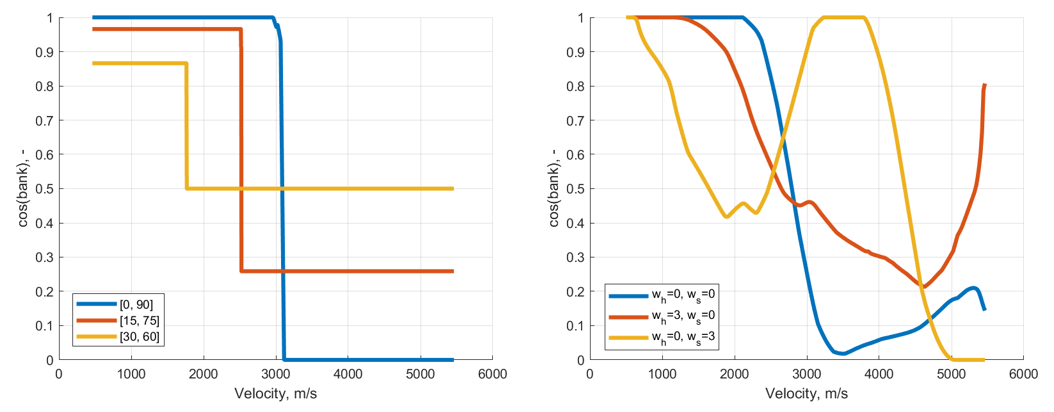
\includegraphics[width=1\textwidth]{ddp/comparison_controls}
	\caption{The profiles from deterministic optimal control (left) exhibit the well known bang-bang structure of altitude optimal trajectories. In comparison, the robust control histories (right) exhibit significantly behavior depending on the weights applied. Note that a significant amount of saturation of the reference control still exists in each of the robust reference designs.}
	\label{fig_control_comparison}
\end{figure}
Figure~\ref{fig_control_comparison} shows the resulting control profiles for the six cases. The altitude-optimal controls resulting from standard optimal control exhibit the well known bang-bang profile while the robust optimal control profiles are quite varied depending on the weights selected. For pure mean optimization, the result is somewhat similar to the bang-bang profiles, but retains margin at high velocities and has a slower transition to the lift up ($u=1$) orientation. An interesting feature of the robust profiles is that saturation still occurs at some velocities. One perspective is that the optimal amount of margin is a quantity that varies along the trajectory, which suggests using a fixed margin will produce inferior results.

%A key observation is that saturation still occurs to some extent in these robust optimal trajectories. Margin is preserved only at key velocities, while at other times the distribution is allowed to grow in order to fly full lift up and raise the terminal altitude. Methods that incorporate chance constraints on the control in order to reduce saturation cannot accomplish this.

For each case, a Monte Carlo simulation with 2000 sample trajectories is conducted to evaluate the performance of each reference. The samples are drawn using Latin Hypercube sampling. The results are summarized in Tables~\ref{table_deterministic}-\ref{table_robust}. Case 1 preserves no margin at all, and as a result has the highest nominal terminal altitude of the three cases. This translates into the highest mean altitude of the three cases, despite the lack of margin. However, the lack of margin causes poor range control performance in dispersed trajectories, leading to unacceptably large range errors. As the amount of control margin increases in Cases 2 and 3, the range errors drop dramatically while the mean altitude also decreases. The 3$\sigma$-low altitudes display non-monotonic behavior with respect to bank margin because the mean altitude loss may be offset by the reduction in altitude deviation. This is true for Case 2, which has a higher 3$\sigma$-low altitude relative to Case 1. In Case 3, the drop in mean altitude is greater than the drop in the 3$\sigma$-low altitude because the altitude deviation has decreased further. 

Case 4 ($ w_h=w_s=0 $) optimizes the mean altitude with knowledge of the problem uncertainty and guidance gains and indeed produces the highest mean altitude of all six cases. Case 5 ($ w_h=3,w_s=0 $) adds additional weight to the altitude standard deviations, which resulted in a 500 meter increase to the 3$\sigma$ low altitude despite a 300 meter drop in mean altitude relative to Case 4. Case 5 has the highest 3$\sigma$-low altitude of the six cases, with more than a kilometer increase over the best of the three profiles designed without incorporating uncertainty. Case 6 ($ w_h=0, w_s=3$) places no weight on altitude standard deviation, but weights range errors heavily, and produces a dramatic decrease in 3$\sigma$ range errors as a result. It has the lowest range error of the six cases, and compared to the large margins of case 3, still produces a higher 3$\sigma$-low altitude.

This demonstrates the applicability of optimal control under uncertainty to designing robust reference trajectories. Additionally, the flexibility of the weights allows the trajectory designer to trade between range errors and altitude performance to the extent that the reference trajectory can alter closed-loop performance. 
\begin{table}[h!]
	\centering
	\caption{As the bank angle margin is increased during the reference trajectory design, range errors decrease dramatically at the expense of a loss in mean altitude. The low end of the altitude distribution is non-monotonic because adding margin can result in a smaller standard deviation, and offset the mean loss (as in Case 2) until the mean loss is too great (as in Case 3).}
	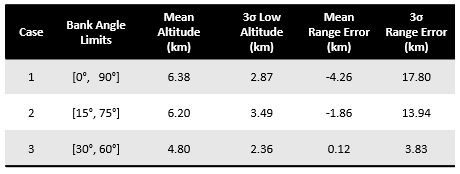
\includegraphics[width=0.75\textwidth]{ddp/table_deterministic}
	\label{table_deterministic}
\end{table}
\begin{table}[h!]
	\centering
	\caption{The trajectories designed with knowledge of the problem uncertainty can outperform Cases 1-3 in each column by appropriate choice of the weights.}
	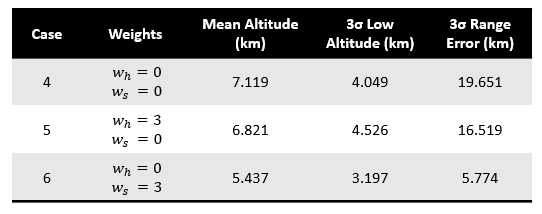
\includegraphics[width=0.75\textwidth]{ddp/table_robust} %
	\label{table_robust}
\end{table}
%Figures~\ref{fig_robust_alt}-\ref{fig_robust_range} show the estimated $3\sigma$ deviations around the mean as well as the sigma point trajectories for scenario 1.
%\begin{figure}[h!]
%	\centering
%	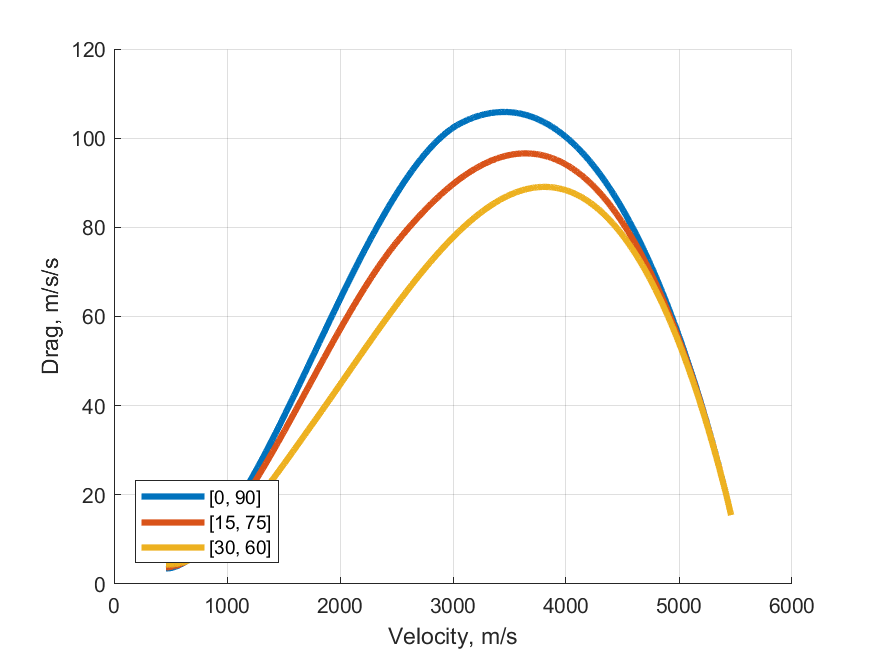
\includegraphics[width=1\textwidth]{ddp/matlab/NominalDrag}
%	\caption{Reference drag profile for each of the four scenarios in Table~\ref{table_comparison}.}
%	\label{fig_drag}
%\end{figure}
%\begin{figure}[h!]
%	\centering
%	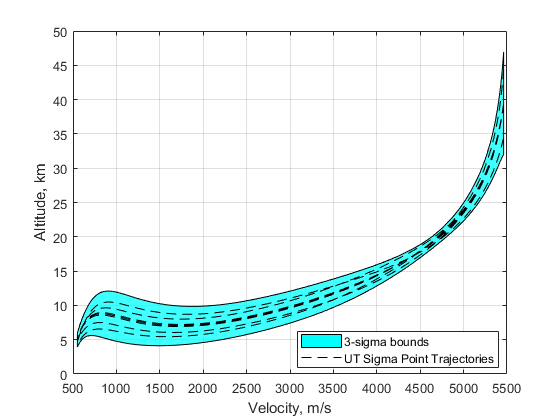
\includegraphics[width=1\textwidth]{ddp/matlab/RobustTrajAlt}
%	\caption{Dispersed altitude performance for scenario 1.}
%	\label{fig_robust_alt}
%\end{figure}
%\begin{figure}[h!]
%	\centering
%	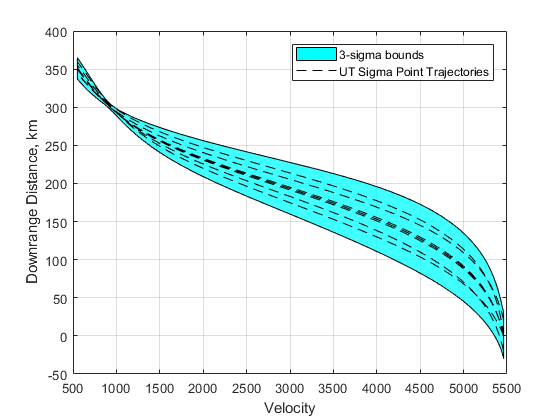
\includegraphics[width=1\textwidth]{ddp/matlab/RobustTrajRange}
%	\caption{Dispersed range performance for scenario 1.}
%	\label{fig_robust_range}
%\end{figure}


\subsection*{Standard Deviation Weighting Study}
From the previous section it is evident there exists a design space where weights on deviations produce superior results to simply optimizing the mean altitude when tail behavior of the distribution is important. This section investigates the extent to which weighting the standard deviations can alter the trajectory performance. The optimal control problem is solved for a variety of weights. The results are summarized in Fig.~\ref{fig_weight_sweep}. Again the advantages of weighting the standard deviations compared with optimizing only the mean are made clear. Comparing $w_h=w_s=0$ with, e.g., $w_h=1,\,w_s = 1$ demonstrates that a 50\% reduction in the standard deviation of downrange distance can be obtained with no loss in the low end of the terminal altitude distribution. Additionally, we can numerically determine the trade between terminal altitude and downrange robustness. The minimum downrange standard deviation achieved ($w_h=0,w_s=3$) was 2.1 km, nearly a 70\% reduction from the mean optimization with $\sigma_s(v_f)=6.7$ km. These trajectories show clear improvements with no change to the guidance gains - simply a different trajectory through the atmosphere is used to improve the results.

%This also highlights the power of the approach as a design tool. If, for example, the $3\sigma$-low terminal altitude is not sufficient for any values of $w_h,\,w_s$, then some aspect of the mission must be reconsidered: increase the terminal velocity, increase the vehicle $L/D$, decrease ballistic coefficient, etc. If a $3\sigma$-low altitude limit is known, then only points that satisfy this limit are considered, and the point with the lowest downrange error may be selected. 

Furthermore, this was achieved using constant feedback gains; this suggests more sophisticated methods of generating gains, such as the Linear-Quadratic Regulator, Apollo influence coefficients, or joint optimization of the feedback gains in the optimal control problem, could produce even greater synergistic improvements to the trajectory design. 
%\begin{figure}[h!]
%	\centering
%	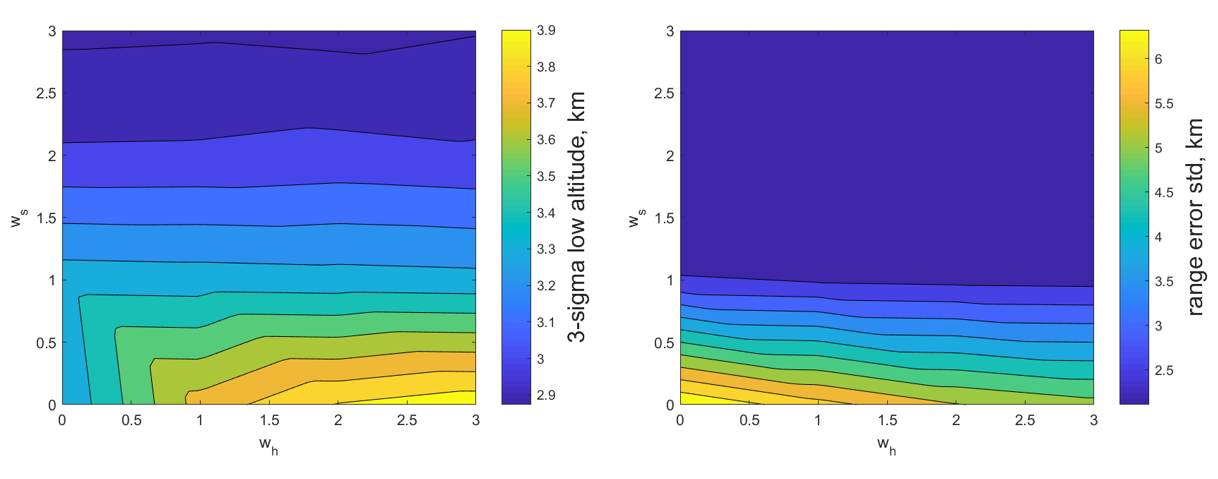
\includegraphics[width=1\textwidth]{ddp/weight_sweeps}
%	\caption{Contours of the unscented transform estimated 3$\sigma$ low altitude (left) and downrange distance standard deviation (right) as a function of the weights $w_h$ and $w_s$. The total range of low altitudes variations is about 1 km, while range errors rapidly improve as $w_s$ is raised to 1, and diminishing returns occur for larger values.}
%	\label{fig_weight_sweep}
%\end{figure}
\begin{figure}[h!]
	\centering
	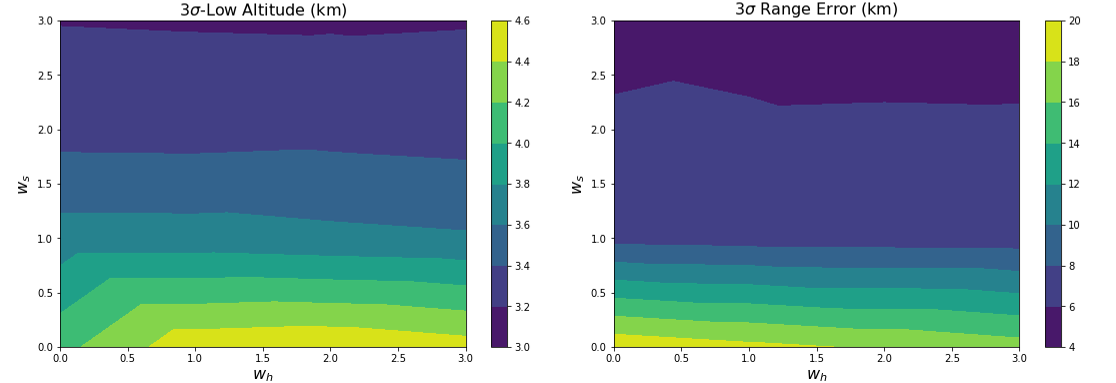
\includegraphics[width=1\textwidth]{ddp/weight_sweeps_mc}
	\caption{Contours of the Monte Carlo 3$\sigma$ low altitude (left) and 3$\sigma$ downrange distance error (right) as a function of the weights $w_h$ and $w_s$. The total range of low altitudes variations is about 1.5 km, while range errors rapidly improve as $w_s$ is raised to 1, and diminishing returns occur for larger values.}
	\label{fig_weight_sweep}
\end{figure}
%\begin{figure}[h!]
%	\centering
%	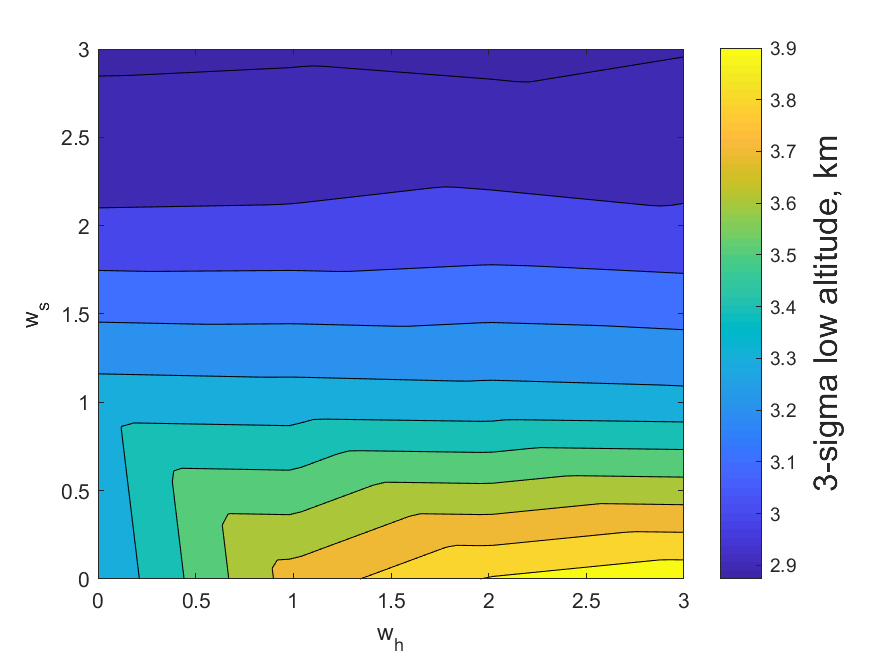
\includegraphics[width=0.75\textwidth]{ddp/matlab/ClosedLoopAltitude}
%	\caption{Contours of the unscented transform estimated 3$\sigma$ low altitude for different weights. As one should expect, this quantity is maximized for $w_h=3,\,w_s=0$, and drops as the weight on range errors increases. Red circles indicate the weights for which the optimal control problem was solved.}
%	\label{fig_weight_sweep_altitude}
%\end{figure}
%\begin{figure}[h!]
%	\centering
%	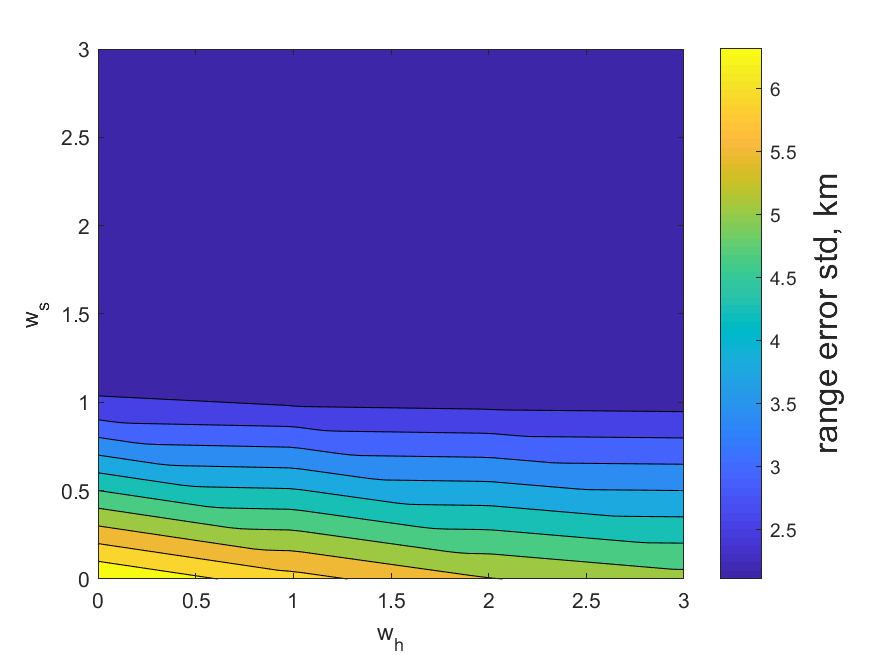
\includegraphics[width=0.75\textwidth]{ddp/matlab/ClosedLoopRangeError}
%	\caption{Contours of the unscented transform estimated downrange standard deviation. Range error rapidly improves as $w_s$ is raised to 1, and diminishing returns occur for larger values. Red circles indicate the weights for which the optimal control problem was solved.}
%	\label{fig_weight_sweep_dr}
%\end{figure}
%\begin{figure}[h!]
%	\centering
%	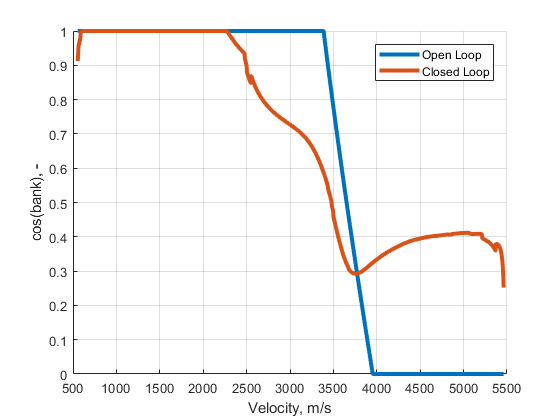
\includegraphics[width=1\textwidth]{ddp/control}
%	\caption{Both solutions display a lower lift segment at high velocities before transitioning to a full lift up arc until the terminal velocity is reached. The primary difference is the closed-loop control leaves substantial margin for feedback control early on until the trajectory errors have been reduced. Once parametric uncertainty is introduced, margin is expected to be required throughout the trajectory.}
%\end{figure}



%\subsection{open-loop vs closed-loop}
%The problem is solved with the weights $w_h = 0.001$, $w_s = 0.01$ and assuming the initial state covariance $\cov = \mathrm{diag}([2500^2,0.25^2,1000^2])$. In the closed-loop scenario, drag, flight path angle, and range-to-go are the feedback states, and the feedback gains are constants $[0.1, -50, 0.1]$. 
%
%\begin{figure}[h!]
%	\centering
%	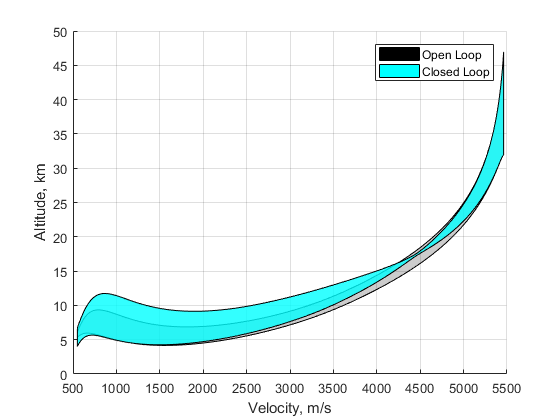
\includegraphics[width=1\textwidth]{ddp/altitude}
%	\caption{The mean altitude remains high but the controller induces additional altitude variance in order to track the downrange distance.}
%	\label{fig_alt}
%\end{figure}
%\begin{figure}[h!]
%	\centering
%	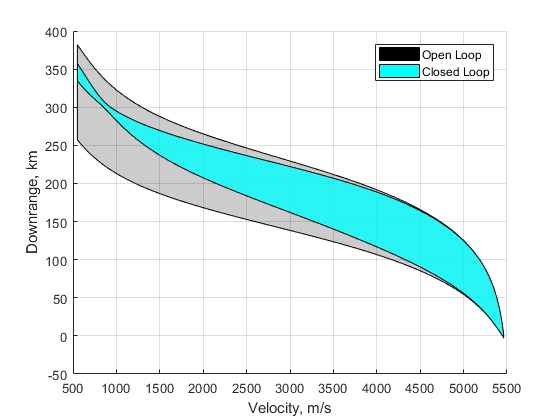
\includegraphics[width=1\textwidth]{ddp/downrange}
%	\caption{The controller produces a substantial reduction in downrange error at a small increase to altitude variance.}
%	\label{fig_dr}
%\end{figure}
%\begin{figure}[h!]
%	\centering
%	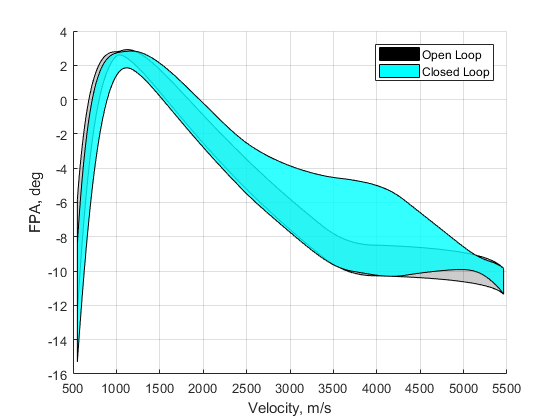
\includegraphics[width=1\textwidth]{ddp/fpa}
%	\caption{Worth noting is the non-monotonicity of the flight path angle variance, which increases substantially during the closed-loop control. The nonlinearity of the trajectory is used to achieve reduced terminal variance in the other state variables.}
%	\label{fig_fpa}
%\end{figure}
%\begin{figure}[h!]
%	\centering
%	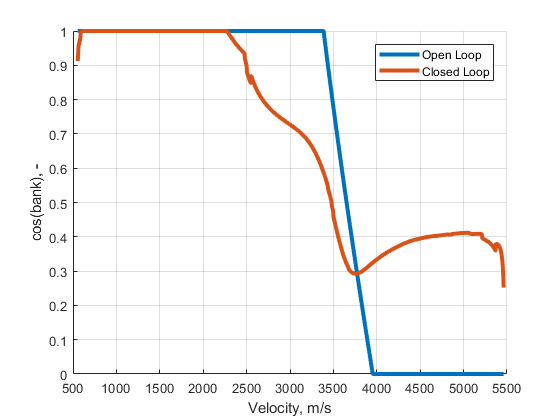
\includegraphics[width=1\textwidth]{ddp/control}
%	\caption{Both solutions display a lower lift segment at high velocities before transitioning to a full lift up arc until the terminal velocity is reached. The primary difference is the closed-loop control leaves substantial margin for feedback control early on until the trajectory errors have been reduced. Once parametric uncertainty is introduced, margin is expected to be required throughout the trajectory.}
%	\label{fig_control}
%\end{figure}

%\subsection{Equal Weight Comparison}
%% Data saved in EqualWeightComparison.mat
%Compare scenarios with the same weights: open-loop, CL with fixed gains, CL with optimized gains. Also add results for flying the open-loop profile but with either/both the fixed gains or the optimized gains. Show that both sets of gains improve the results of course, but the optimized gains are only "optimal" in conjunction with the reference profile - synergy between the two improves the net result.


%\subsubsection*{Uncertainty Quantification Validation}
%Although we have demonstrated that the trajectories designed using the propsed method with UT estimated statistics do translate into improved performance in Monte Carlo simulation, one question remaining is how accurate the unscented transform estimates are relative to the Monte Carlo results. Additionally, could linear propagation suffice in place of the unscented transform? The two objectives of this section are
%\begin{enumerate}
%	\item Verify that the mean and standard deviations computed via Unscented Transform are sufficiently close to MC results
%	\item Demonstrate that in the presence of saturation, linear covariance propagation produces poor estimates
%\end{enumerate}

%Figure~\ref{fig_sweep_errors}
%\begin{figure}[h!]
%	\centering
%	\includegraphics[width=1\textwidth]{ddp/weight_sweep_errors}
%	\caption{The low altitudes are uniformly underestimated, while the range errors show both over- and under-estimates, depending on the weights. }
%	\label{fig_sweep_errors}
%\end{figure}


%\subsection*{LQR and Apollo Gains}
%In this section we investigate the impact of time-varying gains computed via LQR, or using the state of the art modified Apollo gains. 

%\subsection*{Discussion}
%The second order method consistently finds the same solution for open-loop and closed-loop when the gains are not optimization variables. When the gains are also optimized, the initial guess has a large effect on the solution found, suggesting a difficult optimization landscape with many local minima. 

\section*{Conclusion}
%Although a conclusion may review the main points of the paper, it must not replicate the abstract. A conclusion
%might elaborate on the importance of the work or suggest applications and extensions. Do not cite references in the
%conclusion. Note that the conclusion section is the last section of the paper to be numbered. The appendix (if present), funding information, other acknowledgments, and references are listed without numbers

We have presented a new approach to generating robust, altitude-optimal reference trajectories for Mars entry guidance. The entry guidance problem is posed as an optimal control problem with uncertain initial state and parameters. The statistics required to evaluate the objective function are estimated with sample trajectories computed via the unscented transform. Differential dynamic programming is demonstrated to be an effective way to solve the resulting large-scale optimal control problem. By weighting the altitude optimization objective with standard deviations on altitude and downrange distance, entry trajectories robust to the modeled uncertainties are generated. Monte Carlo simulations were conducted to verify the improvement over conventional design techniques based on deterministic optimal control. 
\appendix
\section*{Altitude Rate Feedback Conversion}
There exists a velocity-varying gain $k_{\dot{h}}(v)$ such that $k_{\dot{h}}(v)\delta\dot{h}(v) = k_{\gamma}\delta\gamma\;\forall\,\gamma,\, \dot{h}$.
Proof: 
\begin{align}
\dot{h} &= v\sin\gamma \\
\delta \dot{h} &= v\delta\sin\gamma \\
\delta\sin\gamma &= 2\cos\frac{\gamma+\gamma_r}{2}\sin\frac{\gamma-\gamma_r}{2} \\
\delta\sin\gamma &\approx 
\end{align}
\bibliography{bib}

\end{document}